\documentclass [a4paper,12pt,utf8]{report}
\usepackage [francais]{babel}
\usepackage[utf8]{inputenc}
\usepackage[T1]{fontenc}
\usepackage{url}
\usepackage{graphicx}
\usepackage{color}
\usepackage{amsfonts}
\usepackage{amsmath}
\usepackage{subfig}
\usepackage{rotating}



\setcounter{tocdepth}{1} % ne pas afficher les subsection dans la tableofcontents


\begin{document}

\begin{titlepage}
\begin{center}
{\bf Université Sciences et Technologies - Bordeaux 1} \vspace{0.5cm}\\

{\bf {\large Master 1 Informatique}}\\
{ \emph{Projet de programmation}}\\\vspace{5cm}



{\huge{\bf Génération procédurale de terrains et de planètes}}\\\vspace{1cm}

{\large{\bf{Rapport du 08 avril 2014 :}}}\vspace{1cm}

{\large\bf\it\rm Rapport final
}\vspace{2cm}


\end{center}


\hspace{1cm}\textbf{Réalisé par :}

\hspace{1cm}{Simon CAULE}

\hspace{1cm}{Pierre HUCHANT}

\hspace{1cm}{Solène JOLLY}

\hspace{1cm}{Adrien LAMOUREUX}\\


\hspace{1cm}\textbf{Encadrés par :} Adrien BOUSSICAULT\\

\hspace{1cm}\textbf{Client :} Emmanuel FLEURY\\

\end{titlepage}

\tableofcontents

\begin{titlepage}
\begin{center}
\vspace{5cm}
{\bf {\large Remerciements}} \vspace{3cm}\\
\end{center}
Nous remercions tout d'abord notre encadrant, M. Boussicault, pour l'aide qu'il nous a apporté. \\
Aussi, nous sommes reconnaissants envers notre client, M. Fleury, pour sa disponibilité à répondre à nos questions. \\
Enfin, nous remercions M. Narbel ainsi que l'équipe du LabRI pour l'initiation proposée au Génie Logiciel.


\end{titlepage}

\chapter{Étude de l'existant}

\section{Analyse des algorithmes et méthodes existantes}
La génération procédurale de terrains étant un sujet qui intéresse de nombreux développeurs, il existe un nombre très importants d'algorithmes dans ce domaine. Nous en avons sélectionné une dizaine qui pourront nous \^etre utiles pour ce projet. Nous pouvons les catégoriser de la façon suivante :
\begin{itemize}
\item les bruits ;
\item les fractales ;
\item les raffinements.
\end{itemize}


\subsection{Les bruits}
Un bruit est une application de $\mathbb R^n$ dans $\mathbb R$, on lui fourni
une entrée sur n-dimensions avec coordonnées réelles et il retourne un réel.
Un bruit permet donc d'associer une valeur à chaque point de l'espace.\\

Les bruits dit cohérents possèdent les trois propriétés suivantes :
\begin{itemize}
\item la même valeur d'entrée retournera toujours la même valeur de sortie ;
\item un petit changement dans la valeur d'entrée produira un petit changement dans la valeur de sortie ;
\item un grand changement dans la valeur d'entrée produira un grand changement
dans la valeurs de sortie.\\
\end{itemize}

On peut donc se servir des bruits cohérents pour générer des textures ou
bien des cartes d'élévations, pour cela on fourni en entrée au bruit les
coordonnées de chaque point de la texture ou de la carte d'élévation
et la sortie nous donne la couleur ou l'élévation.\\
Nous allons maintenant présenter les algorithmes des bruits de cellule, de valeur, de Perlin et de simplexe.

\subsubsection{Bruit de cellule}
Le bruit de cellule propose une représentation différente des points dans l'espace. Effectivement, ils sont caractérisés par les points autour d'eux.
Cela signifie qu'un point existant proche du point traité aura plus d'influence sur la valeur de ce dernier.
\paragraph{}
La première étape consiste donc à placer les points existants. Ils sont générés sur une grille 2D de façon pseudo-aléatoire et chaque case de la grille peut contenir un ou plusieurs points (comme illustré dans la figure~\ref{fig:cell-noise}).
La seconde étape est d'intégrer chaque point à traiter sur cette grille puis de comparer la distance entre le point à traiter et ses plus proches voisins.

\begin{figure}[ht!]
    \begin{center}
        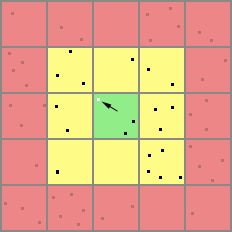
\includegraphics[width=10cm]{resources/cellgrid.png}
        \caption{Grille du bruit de cellule}
        \label{fig:cell-noise}
    \end{center}
\end{figure}

L'élévation du point traité sera donc le résultat du calcul de distance.
\paragraph{}
Il est possible d'obtenir divers résultats selon la méthode de calcul de distances utilisées. Effectivement, il existe plusieurs méthodes valables pour cet algorithme :
\begin{itemize}
 \item Euclidienne
 \begin{equation}
  distance = \sqrt{(x1 - x2)^2 + (y1 - y2)^2}
 \end{equation}
 \item Manhattan
 \begin{equation}
  distance = abs(x1-x2) + abs(y1-y2) 
 \end{equation}
 \item Chebyshev
 \[
    distance= 
\begin{cases}
    |x1-x2|,& \text{si } |y1-y2|\geq|x1-x2|\\
    |y1-y2|,& \text{sinon}
\end{cases}
\]
 \item Quadratique
  \begin{equation}
  distance = (x1-x2)*(x1-x2) + (x1-x2)*(y1-y2) + (y1-y2)*(y1-y2)
  \end{equation}
\end{itemize}

\paragraph{}
L'algorithme prend donc en entrée :
\begin{itemize}
 \item un point à traiter;
 \item une grille 2D;
 \item une méthode de calcul de distances entre points.
\end{itemize}
L'algorithme retourne une valeur caractéristique de la hauteur du point traité.\newline
Plus de détails concernant ce bruit peuvent être trouvés dans ce livre\cite{Eber02}.


\subsubsection{Bruit de valeur}
Le bruit de valeur (value noise), décrit dans le livre
\cite{Eber02} p.70, est généré à partir de 2 choses :\\
\begin{itemize}
\item un générateur pseudo-aléatoire (c'est à dire un générateur qui semble
aléatoire mais qui lorsque on lui donne la même entrée produit toujours la même
sortie) ;
\item une fonction d'interpolation.\\
\end{itemize}

Le générateur pseudo-aléatoire est une fonction discrète, cette fonction
n'est définie que pour les valeurs entières.

\'Etant donné un nombre pseudo-aléatoire pour chaque coordonnée entière d'un
ensemble à n-dimensions, un bruit de valeur peut-être calculé en interpolant les
valeurs entre chacune de ces coordonnées, obtenant ainsi une application
de $\mathbb R^n$ dans $\mathbb R$.

Si l'on prend l'exemple du bruit de valeur sur une dimension, avec le
générateur pseudo-aléatoire, on obtient une valeur pour chaque coordonnée
entière sur l'axe des X, donc une fonction définie sur $\mathbb N$.
Ensuite, on interpole les valeurs entre chaque entier pour définir une nouvelle fonction prenant en paramètres
un réel. L'interpolation nous permet donc de passer d'une fonction définie sur
$\mathbb N$ à une fonction définie sur $\mathbb R$. La fonction ainsi obtenu
est notre bruit de valeur (voir exemple sur les figures ~\ref{fig:noise_function} et ~\ref{fig:noise_function2}).

\begin{figure}[htp]
  \centering
  \subfloat[Valeurs aléatoires pour chaque point de coordonnée entière.] {
        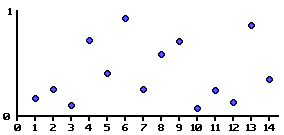
\includegraphics[width=8cm]{resources/noise-function.png}
        \label{fig:noise_function}
  }
  \subfloat[Bruit de valeur généré en interpolant les points.] {
        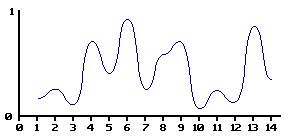
\includegraphics[width=8cm]{resources/noise-function2.png}
        \label{fig:noise_function2}
  }
  \caption{Bruit de valeur sur une dimension (images provenant de
    \cite{PerlinWeb}).}
\end{figure}

Il est possible d'utiliser un grand nombre de fonctions d'interpolations
(linéaire, cosinusoidale, cubique, etc) avec, pour chacune, des rendus
différents (pour un rendu cohérent et détaillé, il est préférable d'utiliser des
valeurs issues d'une interpolation cubique).

\subsubsection{Bruit de Perlin}
Le bruit de Perlin ou bruit gradient ressemble au bruit de valeur mais
diffère par le fait qu'au lieu d'utiliser des nombre pseudo-aléatoire pour chaque
coordonnée entière, on utilise des vecteurs de gradient.

Du fait de sa complexité il ne sera pas décrit de façon détaillée dans ce document.

Pour plus d'information, se référer au livre \cite{Eber02} p.72.

La bibliothèque Libnoise (que nous présenterons dans la section \ref{ref:libnoise} à la page \pageref{ref:libnoise}) propose une implémentation en C++ du bruit de Perlin.

\subsubsection{Bruit de simplexe}
Le bruit de simplexe (simplex noise) est une amélioration faite par Ken Perlin
du bruit de Perlin originale.
Il a, entre autre, l'avantage d'être moins coûteux en complexité pour des dimensions supérieures à trois.

Du fait de sa complexité il ne sera pas décrit de façon détaillé dans ce document.

Pour plus d'informations, se référer à l'article de Gustavson ~\cite{SimplexNoise}
qui décrit précisément le fonctionnement de ce bruit.

\subsubsection{Amplitude et fréquence}
Pour simplifier les explications, nous avons supposé, dans les sections précédentes, que les générateurs
pseudo-aléatoire nous fournissait une valeur pour chaque coordonnée entière,
or dans la réalité la distance entre chaque valeur définie par ces générateur
est définie par l'utilisateur, c'est ce que l'on appelle le \emph{pas}.

La fréquence d'un bruit est définie par $1 / pas$.\\

De plus pour chaque générateur pseudo-aléatoire, la différence entre la
valeur maximum et la valeur minimum possible en sortie nous permet de définir
\emph{l'amplitude} de notre bruit.\\

 Pour chaque bruit \emph{l'amplitude} et la \emph{fréquence} désirés
peuvent donc être spécifiés par l'utilisateur permettant ainsi d'obtenir des
bruits différents selon le résultat attendu.\\

La figure ~\ref{fig:noise-freq-ampl} illustre \emph{l'amplitude} et le \emph{pas}
(wavelength) d'une fonction de bruit.\\

\begin{figure}[ht]
  \centering
  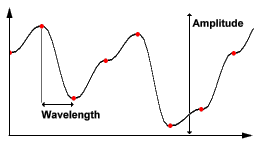
\includegraphics{resources/noise-freq-ampl.png}
  \caption{Fréquence et amplitude d'une fonction de bruit (image provenant de
    \cite{PerlinWeb}).}
  \label{fig:noise-freq-ampl}
\end{figure}


\subsection{Les fractales}
Dans le livre \cite{Eber02} p. 429, une fractale est définie comme un objet
géométriquement complexe, dont la complexité provient de la répétition
d'une forme donnée sur diverses échelles.

On peut voir les fractales comme une nouvelle forme de symétrie qui
s'exprime par le fait qu'un objet reflète la même forme vu sous
différentes échelles.

Pour illustrer cette symétrie on peut penser par exemple au réseau sanguin.
Observé à différents niveaux de prévision, que ce soit les artères, les veines
ou bien les capillaires, ont retrouve toujours la même structure géométrique.

Beaucoup de phénomènes naturels sont fractals, les montagnes, les rivières par
exemples. Elles sont donc très intéressantes pour créer des cartes d'élévation,
et permette de générer de façon procédurale des reliefs revêtant un aspect
naturel.\\

Les figures ~\ref{fig:mandelbrot} et ~\ref{fig:julia} (respectivement l'ensemble de Mandelbrot et l'ensemble de Julia)
ont été générées à partir de fractales. On remarque aisément la présence d'un
même motif répété à différentes échelles.\\

\begin{figure}[htp]
  \centering
  \subfloat[Ensemble de Mandelbrot] {
        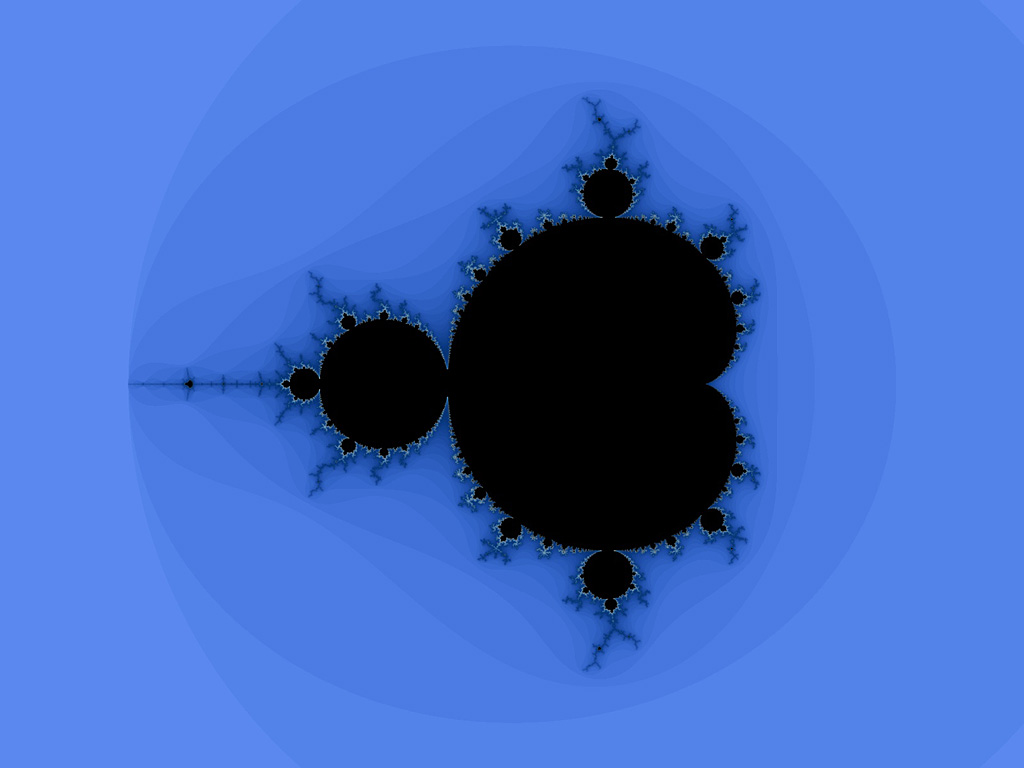
\includegraphics[width=8cm]{resources/mandelbrot.jpg}
        \label{fig:mandelbrot}
  }
  \subfloat[Ensemble de Julia] {
        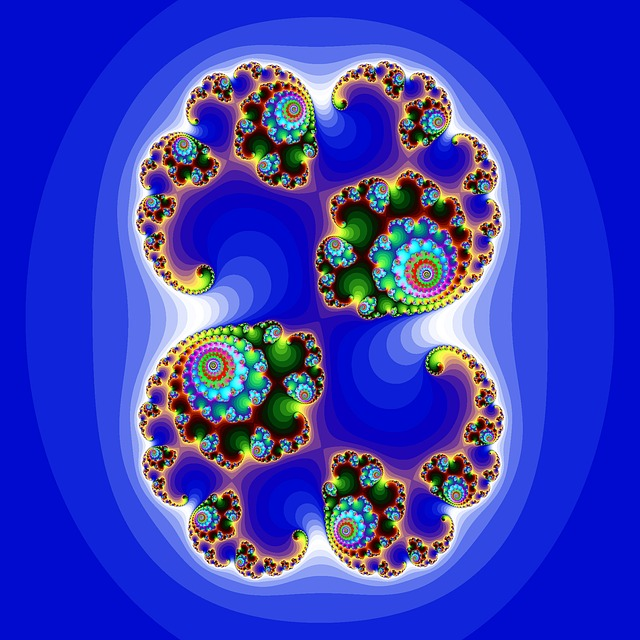
\includegraphics[width=8cm]{resources/julia.jpg}
        \label{fig:julia}
  }
  \caption{Figures géométriques générées à partir de fractales.}
\end{figure}

%% Les méthodes fractales utilisent les propriétés des formes fractales. Une forme fractale est un ensemble cohérent qui aura exactement la m\^eme structure quelque soit l'échelle utilisée. Dans notre projet, ces formes permettent deux choses :
%% \begin{itemize}
%% \item étant cohérente, une fractale représente un seul \og type de zone\fg\ ce qui permettent un rendu réaliste. Par exemple, une fractale représentant une montagne (hauteurs élevées) ne pourra pas présenter au milieu de sa structure un creux inattendu (hauteurs faibles) ;
%% \item le terrain généré garde la m\^eme apparence lorsque l'utilisateur utilise les fonctions de zoom. 
%% \end{itemize}

%% Certaines méthodes, dérivant des méthodes fractales, sont appelées \og multi-fractales\fg\ . Ces dernières offrent la possibilité de créer plusieurs entités fractales distinctes mais cohérentes. Le principe est de générer une première carte renseignant uniquement la hauteur de certains points puis d'intégrer les fractales adéquates selon la hauteur des points. Par exemple, admettons que nous travaillions sur cette carte d'élévations (pour mémoire, blanc = hauteur élevée, noir = hauteur faible) :
%% \begin{figure}[h!]
%%     \begin{center}
%%         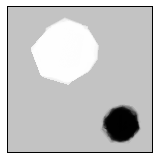
\includegraphics{resources/multi_fractales.png}
%%         \caption{Carte d'élévations factice}
%%         \label{multi-fractales}
%%     \end{center}
%% \end{figure}
%% nous pouvons nettement distinguer trois \og types de zones\fg\ distincts : une zone plane et homogène (grise), une zone élevée (blanche) et une zone basse (noire). Un algorithme multi-fractal appliqué à cette carte créerait trois fractales (une par zone) et des jonctions cohérentes entre les trois fractales. Ceci permet d'obtenir un terrain final cohérent sans être monotone.

Nous allons maintenant présenter les algorithmes des méthodes fractales suivantes : déplacement du point du milieu, diamant-carré et mouvement brownien fractionnaire.

\subsubsection{Déplacement du point du milieu (midpoint displacement)}
Cet algorithme a été introduit dans le livre \cite{Four82}, il prend en entrée
une carte d'élévation carrée vide et génère une élévation
pour chaque entrée de la grille.\\

L'algorithme commence par assigner une valeur aléatoire aux quatre cases
représentant les coins de la grille carrée.

Puis l'élévation du point du milieu de la grille est calculée en faisant
la moyenne des élévations des quatre coins auquel on ajoute une valeur
aléatoire.

Ensuite l'élévation des point des milieux des quatre côtés du carré est calculée
en faisant la moyenne des élévations des deux coins qui l'entourent.
\\

\`A l'issu de cette étape nous pouvons diviser la grille en quatre carrés
ayant tous une élévation assigné en leurs quatre coins.\\

On répète ensuite les deux étapes suivantes jusqu'à avoir rempli toutes les
cases de la grille :\\

\begin{itemize}
\item Pour chaque carré, calculer le point du milieu en faisant la moyenne
des élévations de ses quatre coins à laquelle est ajouté une valeur aléatoire.

\item Calculer le point du milieu de chaque côté du carré en faisant la moyenne
des élévation des deux coins qui l'entourent.\\
\end{itemize}

\`A chaque itération, on réduit l'amplitude de valeurs possibles pour
le nombre aléatoire généré.\\

La figure~\ref{fig:midpoint-displacement} illustre le déroulement de cet
algorithme pour une grille carrée (le principe est le même pour toutes les formes de grilles).

\begin{figure}[ht]
  \centering
  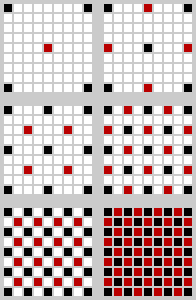
\includegraphics[width=4cm]{resources/midpoint-displacement.png}
  \caption{Déroulement de l'algorithme du déplacement du point du milieu (image
provenant de \cite{FractalTerrainGeneration}).}
  \label{fig:midpoint-displacement}
\end{figure}

\subsubsection{Diamant-carré}
L'algorithme diamond-square a été introduit pour la première fois dans le livre \cite{Four82}. Il s'agit d'une amélioration de l'algorithme de déplacement du point du
milieu. Il diffère de celui-ci dans le déroulement de l'étape du calcul des points
du milieu des côtés.\\

Lors ce cette étape, le point du milieu d'un côté n'est plus calculé seulement
en faisant la moyenne des élévations des deux coins qui l'entourent mais en faisant
la moyennes des élévations des quatre coin du losange englobant le point.\\

De plus une valeur aléatoire est ajoutée à cette moyenne.\\

Les figures~\ref{fig:side-midpoint} et~\ref{fig:side-diamond} illustrent la différence de calcul des points de milieux
des côtés entre l'algorithme de déplacement du point du milieu et celui du
diamant-carré.

\begin{figure}[h]
  \centering
  \subfloat[Algorithme de déplacement du point du milieu.] {
        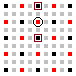
\includegraphics{resources/side-midpoint.png}
        \label{fig:side-midpoint}
  }
  \quad
  \subfloat[Algorithme du Diamant-carré.] {
        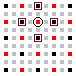
\includegraphics{resources/side-diamond.png}
        \label{fig:side-diamond}
  }
  \caption{Calcul du point du milieu d'un côté (images provenant de
    \cite{FractalTerrainGeneration}).}
\end{figure}



%% Cet algorithme a principalement été conçu pour recréer des montagnes artificielles sur un terrain déjà généré. L'idée est de partir d'un tableau carré à deux dimensions, la taille de ce tableau doit être un multiple de deux plus un (33x33, 65x65, 129x129, etc.). L'algorithme s'exécute en deux étapes.
%% \begin{itemize}
%% \item square : les quatre coins de la matrice sont fixés à la même valeur choisie aléatoirement. La valeur du centre du carré est ensuite calculée à partir de la moyenne des coins à laquelle on aura ajouté une valeur aléatoire ;
%% \item diamond : un diamant étant un losange dont le centre est la valeur initialement fixée, les extrémités du diamant de chaque centre sont moyennées.\\
%% Il faut alors diviser le pas et recommencer la manoeuvre.
%% \begin{figure}[h!]
%%     \begin{center}
%%         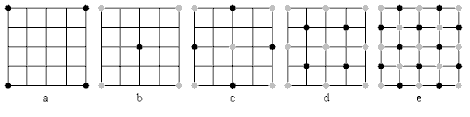
\includegraphics[width=10cm]{resources/square-diamond.png}
%%         \caption{Exemple Diamond-Square}
%%         \label{Diamond-Square}
%%     \end{center}
%% \end{figure}
%% \end{itemize}

\subsubsection{Fractional brownian motion (littéralement : mouvement brownien fractionnaire)}
Cet algorithme sert à appliquer N niveau de bruits sur chaque entrée d'une matrice d'élévation.
Le Fractional Brownian Motion prend en entrée :
\begin{itemize}
 \item un point de la matrice d'élévation;
 \item une méthode de bruits;
 \item une fréquence;
 \item une amplitude;
 \item un nombre d'octave correspondant aux nombres d'itérations successives d'un bruit;
 \item un degré de variation de la fréquence;
 \item un degré de variation de l'amplitude.
\end{itemize}
Il renvoi une valeur représentative de la hauteur du point traité.
\paragraph{}
Les entrées, citées précédemment, servent à configurer l'itération de bruits.
A chaque itération (dépendant du nombre d'octaves), plusieurs événements ont lieu :
\begin{itemize}
 \item mis-à-jour de la fréquence et de l'amplitude (\textit{via} le degré de variation de la fréquence et de l'amplitude);
 \item appel d'une méthode de bruit prennant plusieurs paramètres :
 \begin{itemize}
  \item le point à traiter;
  \item la fréquence;
  \item l'amplitude.
 \end{itemize}
 \item ajout de la valeur de sortie de la méthode de bruit aux précédents résultats.
\end{itemize}
Ainsi, cet algorithme consiste à itérer successivement la même méthode de bruit en faisant varier les paramètres d'entrées de ce dernier.
\paragraph{} 
Cet algorithme peut néanmoins ralentir la conception d'une carte d'élévation à cause du calcul des octaves (et donc des bruits) successifs.
Une description plus détaillé de l'algorithme est disponible dans l'article \cite{Mand68}.


\subsection{Les raffinements}
Les raffinements viennent modifier les hauteurs d'un terrain de façon à faire apparaître des détails liés à l'activité d'érosion, l'activité humaine, la présence de forêts, etc.
Ainsi ils apparaissent comme une sur-couche à ajouter après élaboration du terrain.\newline
Le document suivant \cite{Deus98} présente avec détail comment modéliser un écosystème sur un terrain. Un modèle d'érosion applicable sur la surface d'un terrain est décrit dans ce document \cite{Kell88}.

%%\chapter{Structures de données}

%% http://kiwi.atmos.colostate.edu/BUGS/geodesic/text.html
%% http://sydney.edu.au/engineering/it/~visual/valacon/pdf/papers/JNN06-SphericalSOM.pdf
%% http://www.smos.esa.int/ISEA/gdggs03.pdf
%% http://www.labri.fr/perso/fleury/courses/PdP/MondesVirtuels/terrain_generation/dggriddoc31.pdf
%% http://www.gamedev.net/topic/423908-making-a-mesh-from-a-geodesic-grid/
%% http://www.polycount.com/forum/showthread.php?t=96307

\section{Analyse des logiciels existant}
\subsection{Logiciels libres}
\subsubsection{LibNoise (figure~\ref{fig:libnoise})}
\label{ref:libnoise}

LibNoise~\cite{LibNoise} est une librairie portable et open-source développée en C++
permettant la génération de différents types de bruits cohérents, notamment
le bruit de Perlin (Perlin noise).

\begin{figure}[!ht]
    \begin{center}
        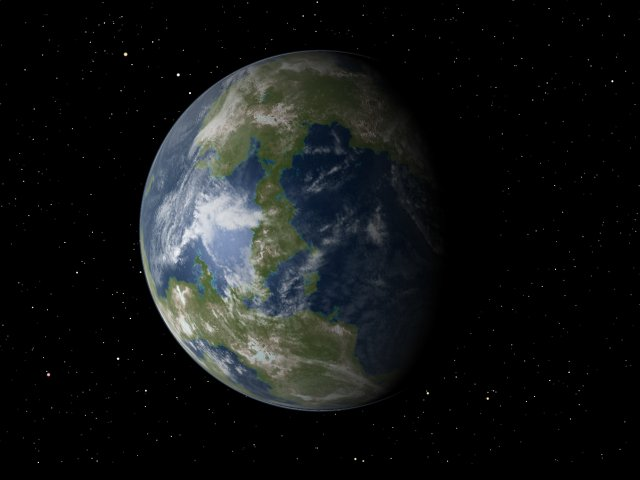
\includegraphics[width=10cm]{resources/libnoise.jpg}
        \caption{exemple de planète générée avec LibNoise rendue avec Celestia}
        \label{fig:libnoise}
    \end{center}
\end{figure}

\subsubsection{Fracplanet (figure~\ref{fig:fracplanet})}

Fracplanet~\cite{FracPlanet} est une application interactive permettant de visualiser et de générer aléatoirement des planètes et des terrains à l'aide de fractales.
Les objets générés peuvent être exportés dans des formats directement
utilisables par POV-Ray ou Blender.
Ce projet a été écrit en C++ et utilise QT et OpenGL.
Il est sous licence GPL.

\begin{figure}[!ht]
    \begin{center}
        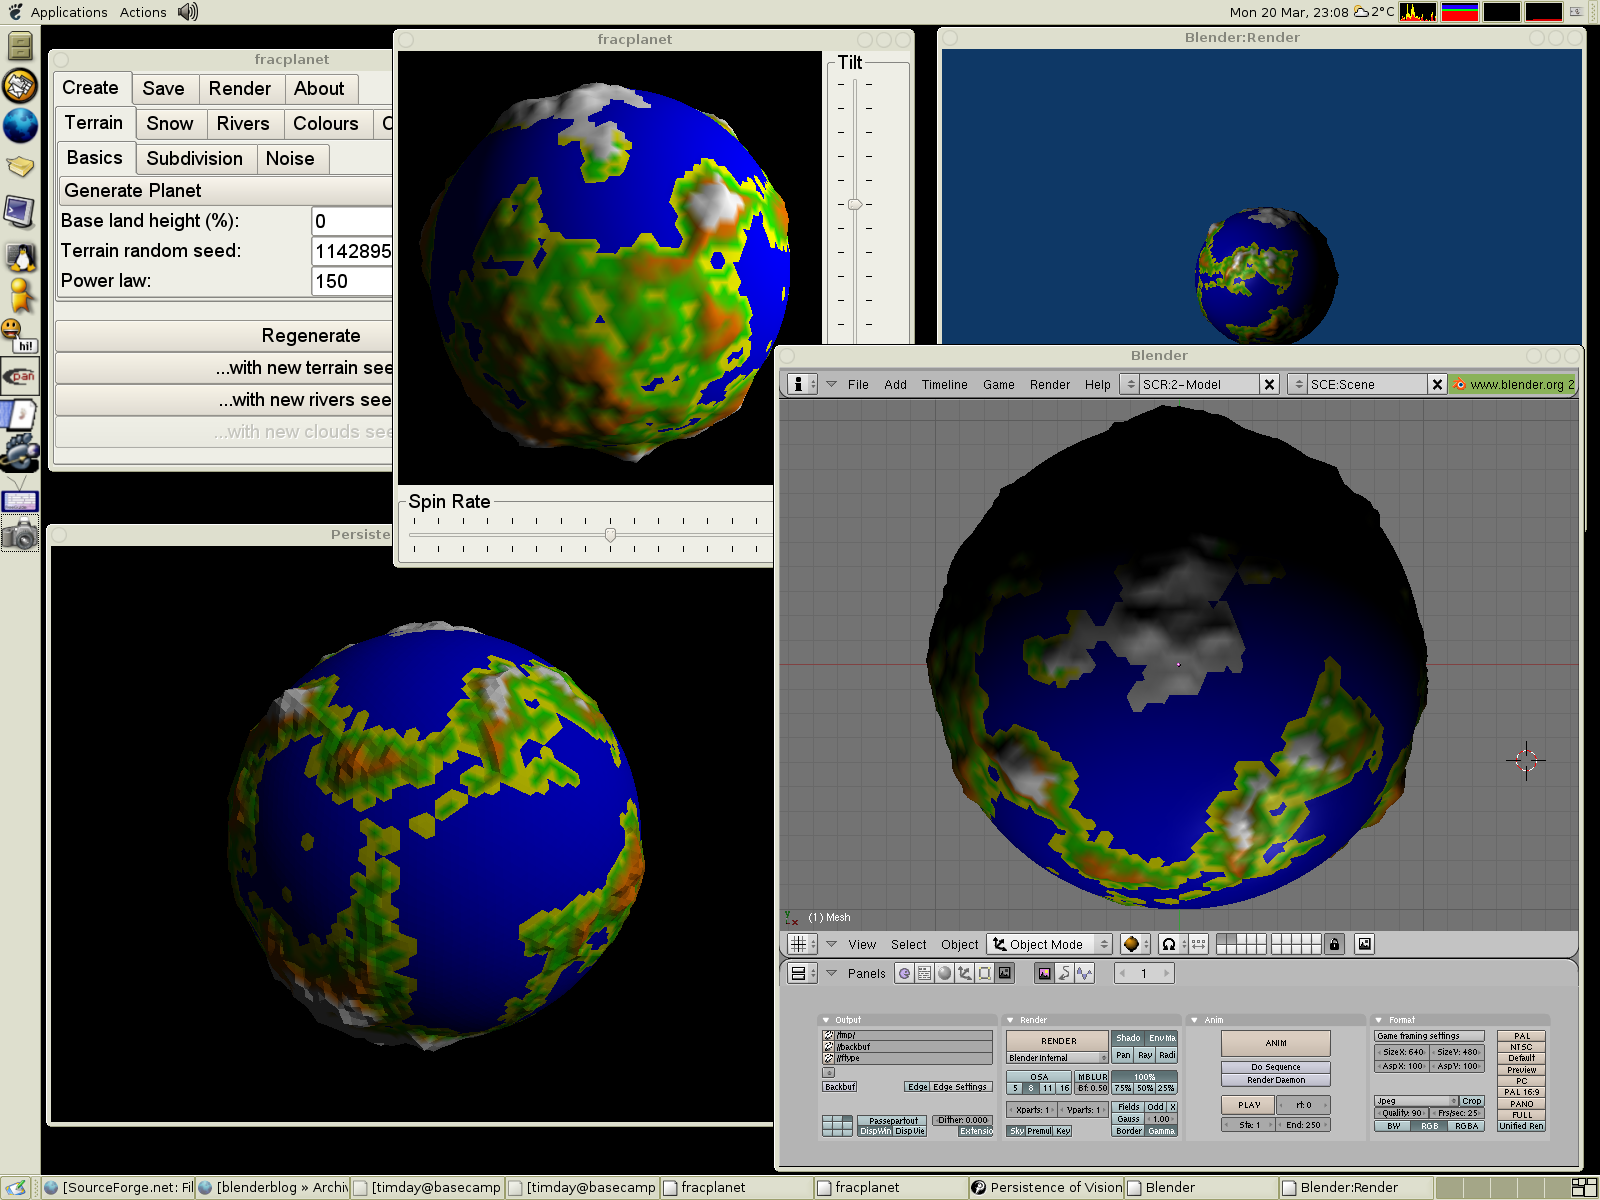
\includegraphics[width=10cm]{resources/fracplanet.png}
        \caption{capture d'écran de FracPlanet}
        \label{fig:fracplanet}
    \end{center}
\end{figure}

\subsubsection{TerraJ (figure~\ref{fig:terraj})}
TerraJ~\cite{TerraJ} est une collection de programmes de génération de terrains fractals et de systèmes solaires (dont Fracplanet) portés du C/C++ vers Java sous licence GPL.

\begin{figure}[!ht]
    \begin{center}
        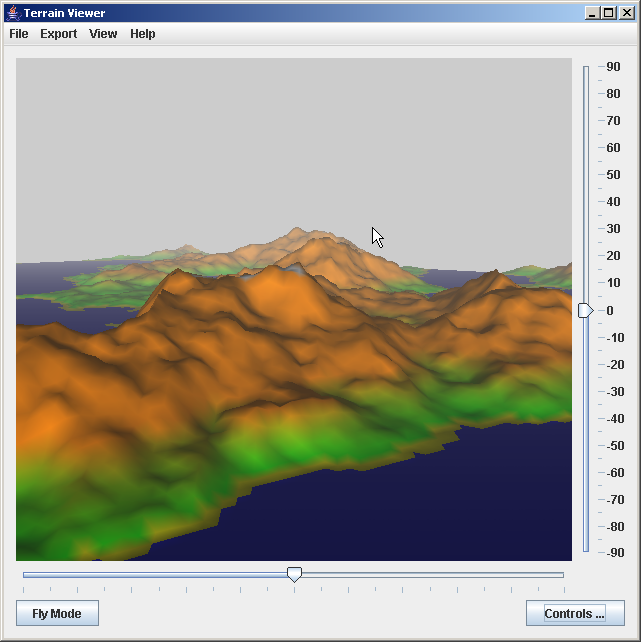
\includegraphics[width=10cm]{resources/terraj.png}
        \caption{capture d'écran de TerraJ}
        \label{fig:terraj}
    \end{center}
\end{figure}

\subsubsection{Terrain.dk (figure~\ref{fig:terrain_dk})}
Le but de ce projet~\cite{largeDetTerrainsURL} open source est de permettre de
visualiser un terrain vaste et détaillé. Les développeurs se sont basé sur deux algorithmes
d'affichages de niveau de détail. Ils utilise "the chunked quadtree structure"
crée par Ulrich ~\cite{Ulrich2002}, mais avec le processus de simplication du
Dr Boer ~\cite{citeulike:623420}.

\begin{figure}[!ht]
    \begin{center}
        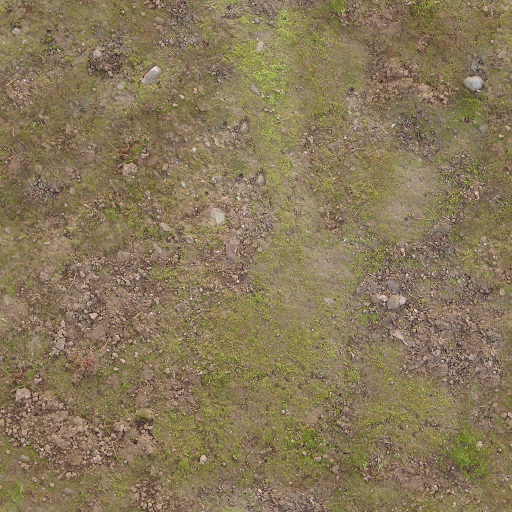
\includegraphics[width=10cm]{resources/terraindk.png}
        \caption{capture d'écran de Terrain.dk}
        \label{fig:terrain_dk}
    \end{center}
\end{figure}

\subsubsection{Irrlicht 3D Engine (figure~\ref{fig:irrlicht})}
Irrlicht 3D Engine ~\cite{irrlicht} est un logiciel libre sous licence zlib, donc compatible avec notre projet. Ce moteur graphique développé par Nikolaus Gebhardt et al. est utilisé dans divers domaines comme la visualisation de planète où les jeux vidéo.
\begin{figure}[!ht]
    \begin{center}
        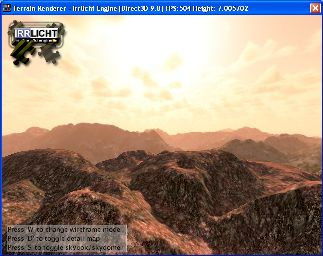
\includegraphics[width=10cm]{resources/irrlicht.jpg}
        \caption{capture d'écran de Irrlicht}
        \label{fig:irrlicht}
    \end{center}
\end{figure}

\newpage
\subsection{Logiciels propriétaires}
\subsubsection{Terragen (figure~\ref{fig:terragen})}
Terragen~\cite{Terragen} est un générateur de terrain très populaire écrit en C++  pour Windows et Mac OS X développé par Planet Side. Il a notamment été utilisé pour la réalisation d'effets spéciaux dans les films : Gatsby le Magnifique (2013), Man of Steel (2013), Tron l'héritage (2010) et bien d'autres.

Il s'agit d'un logiciel propriétaire payant mais il existe aussi une version gratuite aux fonctionnalités limitées pour un usage non commerciale.

\begin{figure}[!ht]
    \begin{center}
        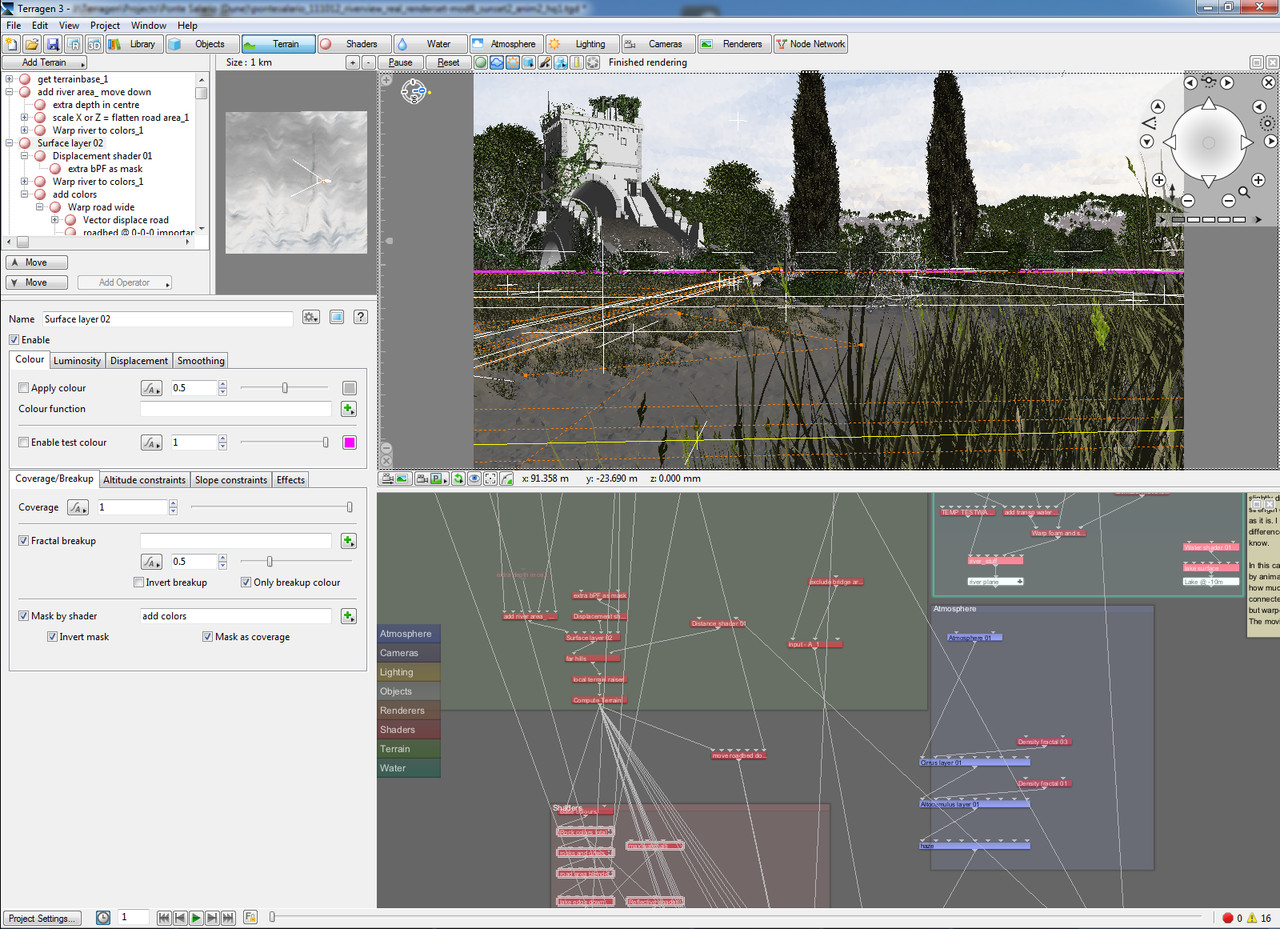
\includegraphics[width=10cm]{resources/terragen.jpg}
        \caption{capture d'écran de Terragen}
        \label{fig:terragen}
    \end{center}
\end{figure}

\subsubsection{MojoWorld (figure~\ref{fig:mojoworld})}
MojoWorld~\cite{Mojoworld} est un générateur de planète propriétaire pour Windows et Mac OS X
commercialisé par Pandromeda Inc.
Il a été crée à l'origine par Ken Musgrave, l'auteur du livre~\cite{Eber02}.

\begin{figure}[!ht]
    \begin{center}
        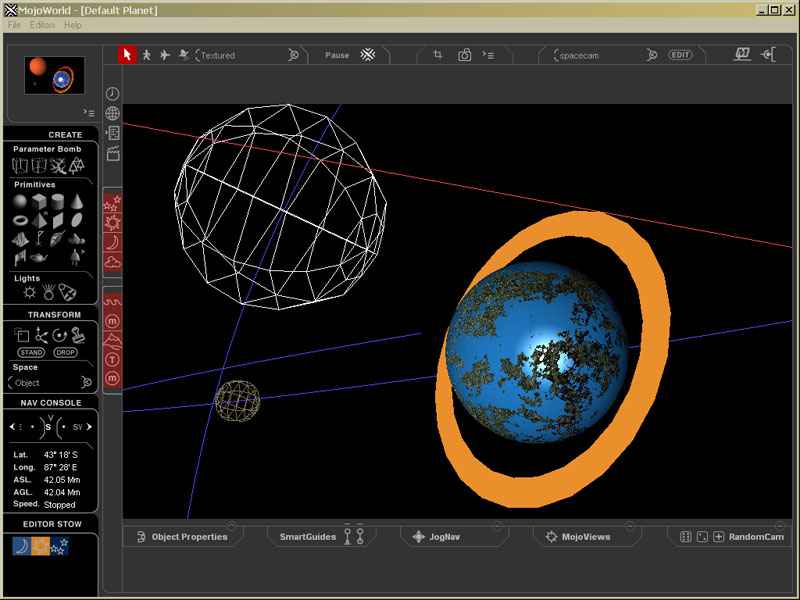
\includegraphics[width=10cm]{resources/mojoworld.jpg}
        \caption{capture d'écran de MojoWorld}
        \label{fig:mojoworld}
    \end{center}
\end{figure}

\subsubsection{Vue (figure~\ref{fig:vue})}
Vue~\cite{Vue} est un générateur de paysages propriétaire pour Windows et Mac OS X.
Il est utilisé pour la création, l'animation et la visualisation d'environnements 3d naturels. Il a été utilisé pour réaliser des effets spéciaux dans de
nombreux films tels que Indiana Jones et le Royaume du crâne de cristal (2008) et Pirates des Caraïbes : Le Secret du coffre maudit (2006).
\begin{figure}[!ht]
    \begin{center}
        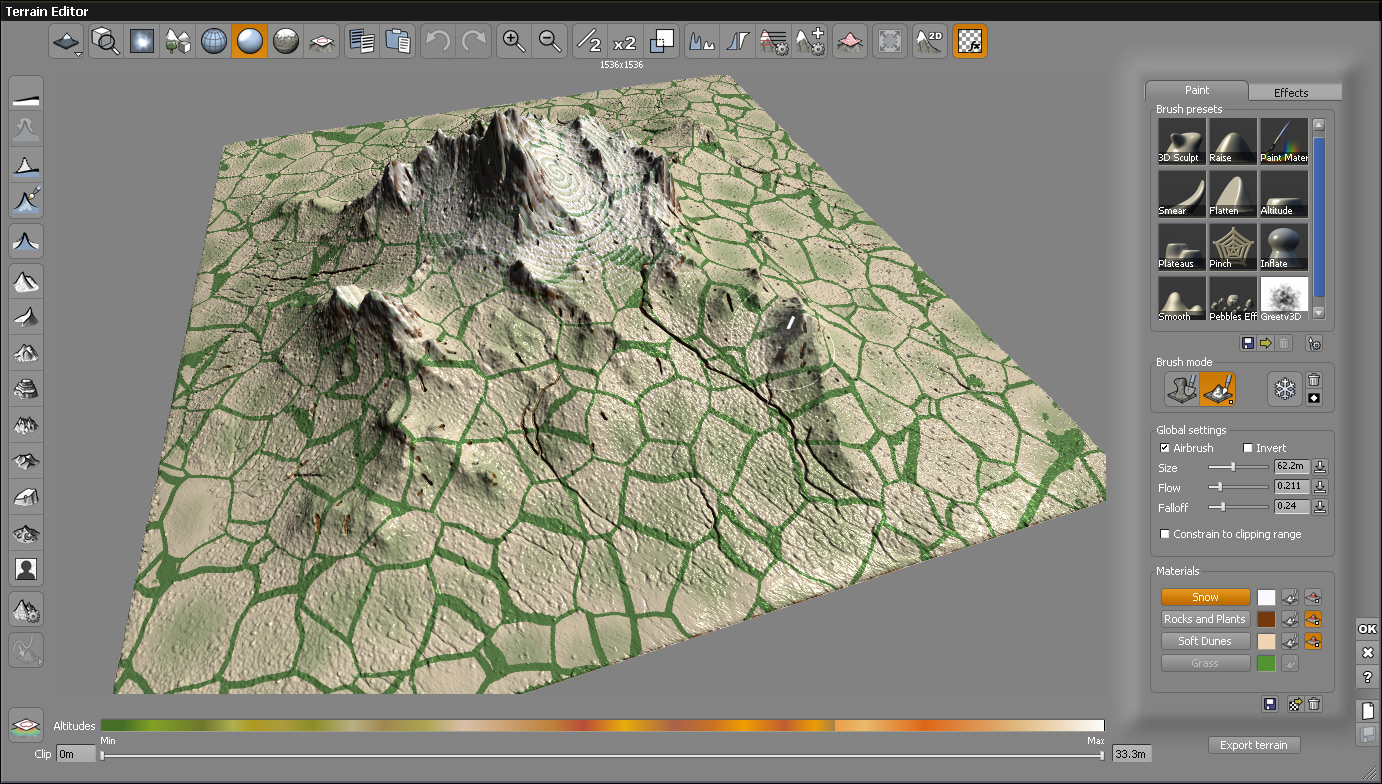
\includegraphics[width=10cm]{resources/vue.jpg}
        \caption{capture d'écran de Vue}
        \label{fig:vue}
    \end{center}
\end{figure}

\subsubsection{Grome (figure~\ref{fig:grome})}
Grome~\cite{Grome} est un logiciel propriétaire de modélisation 3D pour Windows utilisé dans l'industrie des jeux vidéos. Il est développé par Quad Sofware et permet
notamment la génération procédurale de terrain à l'aide de fractales.
\begin{figure}[!ht]
    \begin{center}
        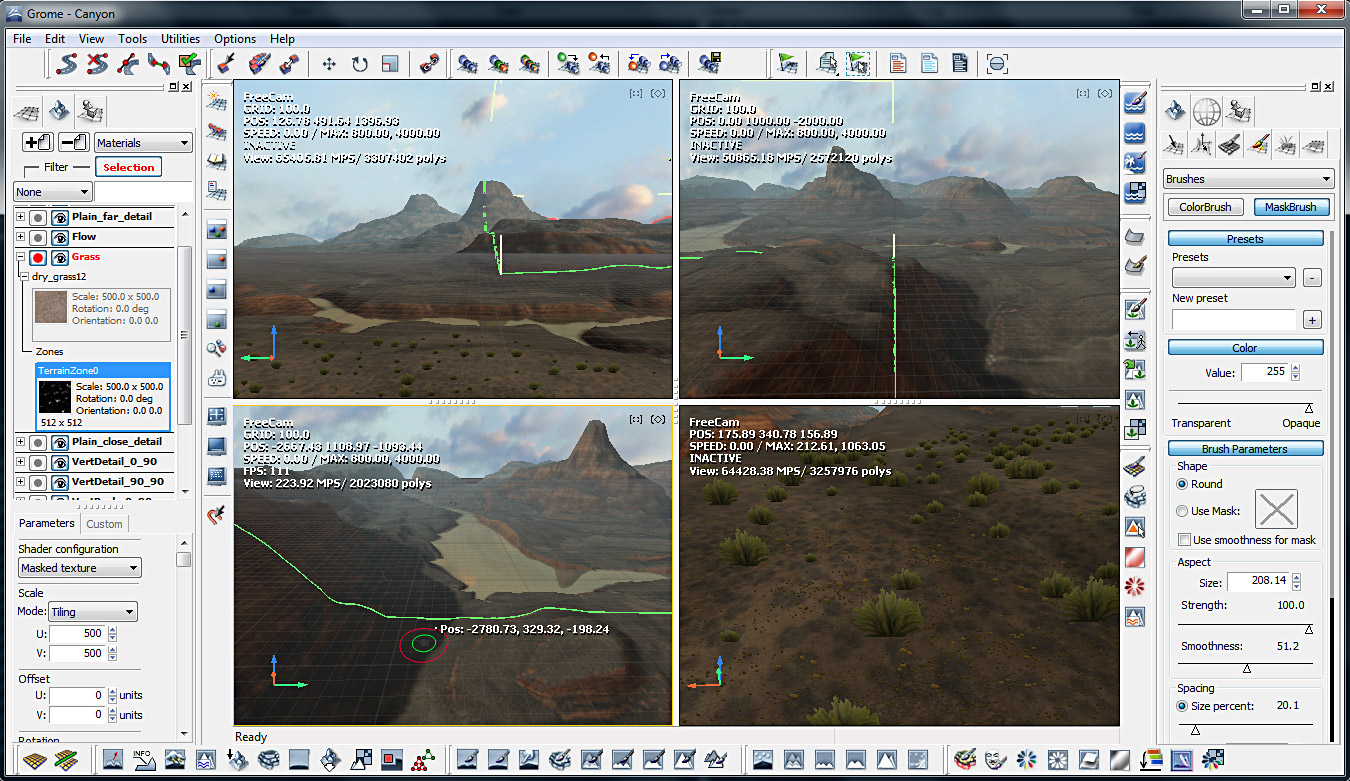
\includegraphics[width=10cm]{resources/grome.jpg}
        \caption{capture d'écran de Grome}
        \label{fig:grome}
    \end{center}
\end{figure}

\chapter{Analyse des besoins}

\section{Objectifs et motivations}
La génération automatique de terrains virtuels est un problème sur lequel
planchent souvent les graphistes et les games designers, car pouvoir créer
 un monde virtuel persistant est une brique de base à de nombreuses
applications. Mais, même si le sujet a été maintes fois traité, il reste un
problème difficile non seulement techniquement à cause de la masse de calculs
 que cela représente mais aussi parce que le rendu final du paysage doit
paraître un tant soit peu réaliste aux yeux des utilisateurs.\\

Le but de ce projet est de créer une bibliothèque permettant la création de
terrains virtuels à partir de méthodes fractales ou de bruits. L'utilisateur de la bibliothèque
pourra réaliser des cartes carrées ou sphériques et disposera d'un choix
conséquent d'algorithmes de génération.
La bibliothèque permettra aussi la visualisation des terrains avec différents
niveaux de détails. \\

\section{Interopérabilité entre la bibliothèque et certains visualisateurs existants}
Il existe de nombreux visualisateurs capables de créer un terrain à partir de cartes d'élévations et / ou de modèles externes.
Ainsi il sera intéressant de combiner le réalisme des cartes d'élévations et des modèles générés avec le rendu proposé par ces visualisateurs. Ceux choisis sont TerraGen3 (référence pour le travail de terrains) et Blender3D (open-source et très efficace pour le travail de modèles). 
Les terrains pourront également être importés. Un visualisateur personnel pourra aussi être amené au projet mais la conception de ce dernier n'est pas une priorité.

\section{Scénario d'exécution}
La figure ci-après présente un scénario d'utilisation de notre
bibliothèque.
L'utilisateur spécifie les paramètres qu'il souhaite aux différentes composantes de
celle-ci. Effectivement, il aura accès aux principales structures (carte d'élévation,
grille, etc).
Les modules de la bibliothèque pourront être utilisés de façon indépendante même s'il
est évident que certains modules doivent être utilisés avant d'autres (e.g : création du terrain avant visualisation).


\begin{figure}[!ht]
    \begin{center}
        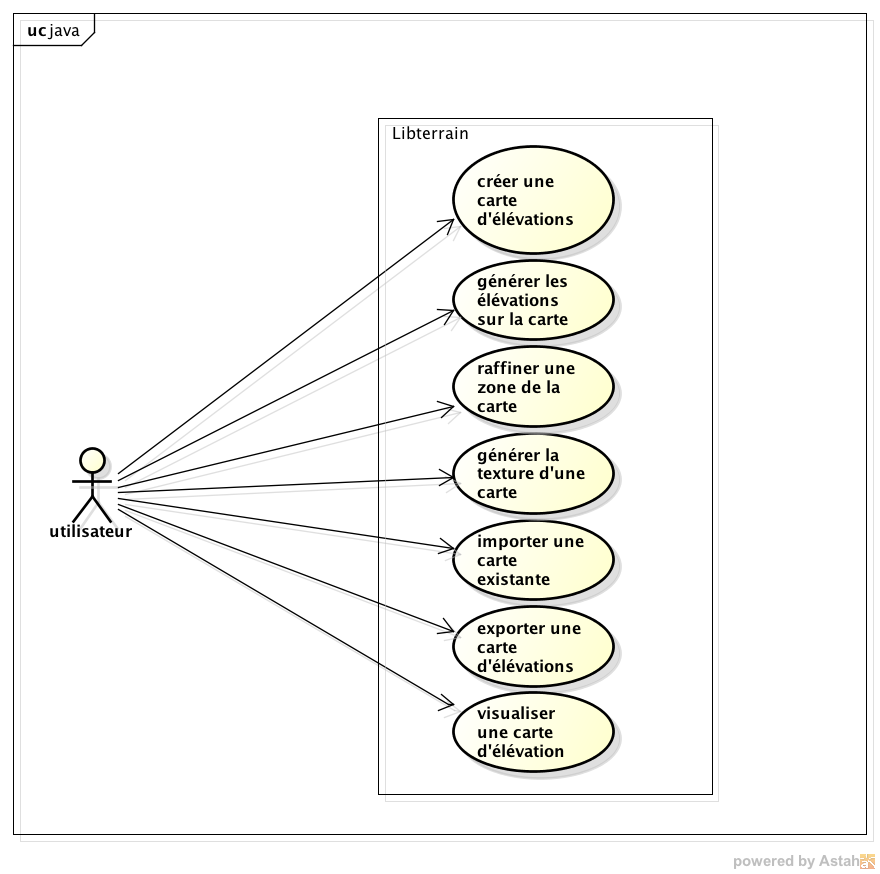
\includegraphics[width=15cm]{resources/use-case.png}
        \label{fig:use_case}
        \caption{Scénario d'exécution}
    \end{center}
\end{figure}

\section{Besoins fonctionnels}

\subsection{Besoins prioritaires}

Ces besoins sont ceux que nous nous engageons à implémenter.

\subsubsection{Structures de données}
La bibliothèque devra proposer deux types de cartes d'élévations :\\
\textbf{sphériques} et \textbf{carrées}.

\subsubsection{Algorithmes de générations de terrains}
Pour permettre la génération d'un terrain, les méthodes suivantes devront pouvoir
 être appliquées sur les cartes d'élévation (les méthodes suivies de la mention [prioritaire] sont celles qui doivent \^etre implémentées en priorité) :\\

\noindent méthodes des fractales :
\begin{itemize}
\item diamond-square ; [prioritaire]
\item midpoint displacement ; [prioritaire]
\item fractional brownian motion ;
\item multi-fractal midpoint displacement.
\end{itemize}
méthodes des bruits :
\begin{itemize}
\item simple noise ;
\item cell noise ;
\item Perlin noise ; [prioritaire]
\item value noise.
\end{itemize}
raffinement par modèles :
\begin{itemize}
\item erosion model.
\end{itemize}

\subsubsection{Raffinement d'un terrain}
S'il souhaite raffiner une zone précise, l'utilisateur pourra la sélectionner (en passant ses coordonnées en paramètres) afin d'appliquer une des méthodes de raffinement (de son choix) sur cette seule zone.

\subsubsection {Génération d'une grille}
Pour les cartes carrées et sphériques, il sera possible de choisir une grille carrée, triangulaire ou hexagonale.

\subsubsection{Importation / exportation}
Les cartes d'élévations pourront être importées et exportées sous forme
d'images (.png, .jpeg) afin d'être lisible par d'autres logiciels
tels que Terragen 3 ou Blender 3D. \newline
Les modèles sont exportés sous format .obj pour être lisible par Blender3D.
Une méthode sera donc conçue pour lire les fichiers importés et une autre pour les concevoir dans le cas d'un export. 

\subsection{Besoins non prioritaires}

\subsubsection{Génération de texture}
Il devra être possible de donner une couleur différente à chaque point de la carte en
fonction de son élévation.

\subsubsection{Implémentation d'un visualisateur 3D}
Génération d'une simple représentation de la carte par rapport à la
carte d'élévation d'origine et du modèle construit par la bibliothèque.

Implémentation d'un zoom pour pouvoir visualiser la carte avec différents niveaux
de détail.


\section{Besoins non fonctionnels}

\subsection{Comportement}

\subsubsection{Performances}
La génération de terrains n'étant pas faite en temps réel, aucune exigence
concernant la vitesse de calcul n'est spécifiée : la qualité du rendu prime sur
le temps d'exécution. Le temps de génération de nos terrains pourra donc \^etre conséquent (de quelques secondes à quelques minutes).\\

Il n'y a pas d'interactivité entre l'utilisateur et le programme pendant l'exécution de ce dernier (le programme peut donc s'exécuter en tâche de fond).\\

\subsubsection{Facilité d'utilisation}
La bibliothèque devra \^etre facile à prendre en main pour l'utilisateur (qui sera un développeur) et devra proposer un maximum d'algorithmes de génération de terrains (parmis ceux qui sont décrits dans les besoins fonctionnels).\\

Il s'agit de développer une bibliothèque et non un logiciel. L'utilisateur
de notre projet est donc un développeur. En conséquence il n'est pas demandé
d'implémenter d'interface graphique pour l'utilisation de la bibliothèque elle-m\^eme, l'utilisateur final pourra, s'il le souhaite, en créer une en s'appuyant sur les différents services proposés par notre bibliothèque.\\

\paragraph{Contraintes :}
Une documentation devra être livrée avec la bibliothèque.

\paragraph{Validation :}
Plusieurs programmes d'exemples illustrant l'utilisation de notre bibliothèque seront livrés.

\paragraph{Portabilité :}
La bibliothèque sera développée pour les plateformes Linux/x86 et devra utiliser
GNU Autotools comme système de construction.

\subsubsection{Contraintes}
Toute utilisation de bibliothèque devra \^etre justifiée afin d'éviter la prolifération des dépendances. La bibliothèque boost ne devra \^etre utilisée qu'en cas d'absolue nécessité.

\subsubsection{Persistance des données de la génération procédurale}
Les exécutions avec les mêmes paramètres (méthodes, graine aléatoire, etc)
doivent fournir le même résultat.

\paragraph{Validation :}
Pour N exécution d'une méthode avec des paramètres identiques, comparer les cartes d'élévations obtenues (sommet par sommet) en vérifiant que les sommets aient les mêmes élévations. 

\subsection{Besoins organisationnels}

\subsubsection{Langage}
L'implémentation sera faite en C++.

\subsubsection{Style de codage}
Le projet devra respecter le style de codage de linux :\\
\url{https://www.kernel.org/doc/Documentation/CodingStyle}\\
\emph{(Dernière visite : 10/02/2014)}
%\subsection{Gestion du temps}
%% TODO diagramme Gant


\subsection{Autres besoins}

\subsubsection{Contraintes légales}
Le projet sera distribué sous Licence Publique Générale Limitée GNU (GNU LGPL).

Nous avons choisi cette licence car c'est une licence de logiciel libre mais
moins contraignante que la GPL. En effet elle autorise à lier un programme
développé sous cette licence à du code non (L)GPL. Il sera donc possible d'utiliser notre bibliothèque dans un programme publié sous une autre licence sans révoquer celle-ci.

\subsubsection{Contraintes d'interopérabilité}
Notre bibliothèque hérite de certains modules provenant de LibNoise. 
Ainsi, il faut respecter les interfaces des modules de Libnoise (typage, etc).
Les cartes d'élévation produites par notre bibliothèque devront être lisible par les visualisateurs
 suivants : TerraGen 3 et Blender 3D.\\
\textbf{Terragen 3} utilise des fichiers au format .TER et les modélise sous forme de terrains.\\
Pour \textbf{Blender 3D}, les traitements en amont sont plus simples car ce logiciel charge
une carte d'élévation (image en niveaux de gris) et sous forme de modèle (fichiers
.obj).
Les configurations se font ensuite depuis Blender 3D.


\chapter{Architecture logiciel}

\section{Architecture globale}

Le projet consiste à construire une bibliothèque permettant de générer plusieurs
types de cartes d'élévations (planes, sphériques) à l'aide de diverses
méthodes (fractales, bruits), et d'exporter ces dernières pour les visualiser sous des logiciels 
comme Terragen et Blender3D.

La figure \ref{fig:class-diagram} présente l'architecture que nous avons imaginé,
elle sera décrite plus en détails dans le chapitre suivant.

\begin{sidewaysfigure}
  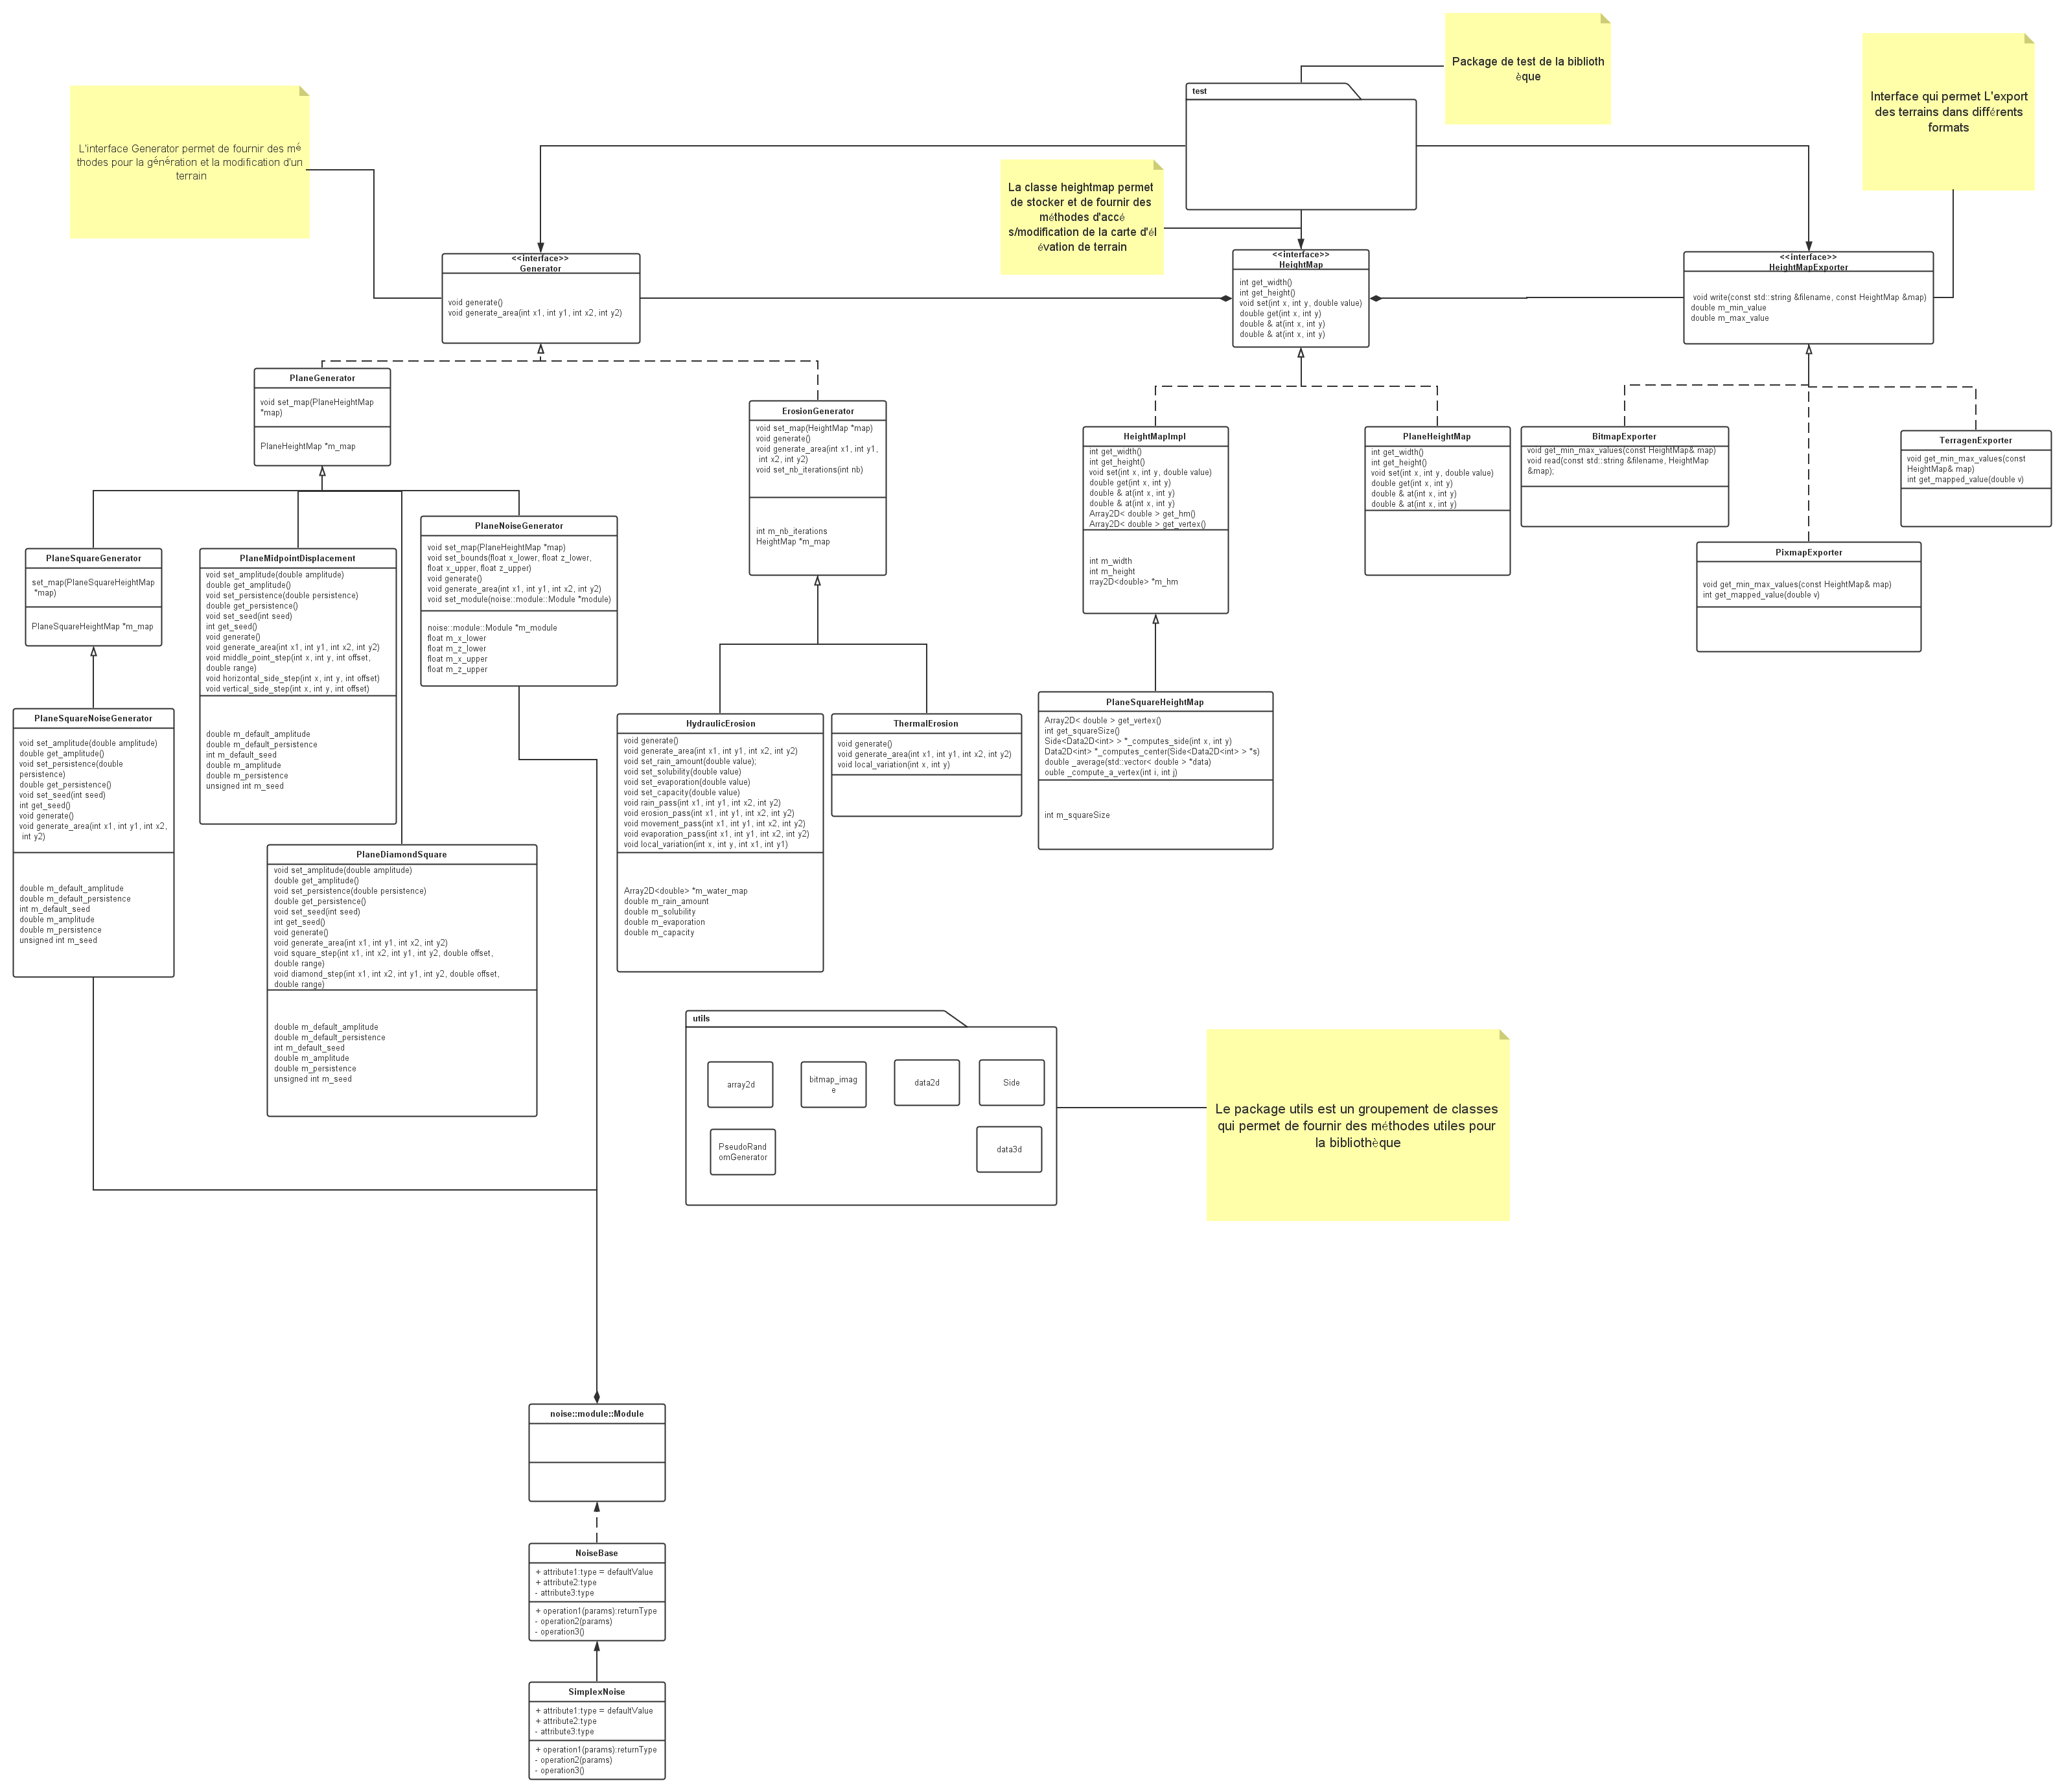
\includegraphics[width=20cm]{resources/Diag_Planetgen_v5.png}
        \caption{Diagramme de classe}
        \label{fig:class-diagram}
\end{sidewaysfigure}

On distingue ainsi 5 modules principaux :
\begin{itemize}
 \item la topologie de la carte d'élévation (classe heightMap);
 \item la génération des hauteurs de la carte;
 \item l'export de la carte;
 \item les classes utilitaires;
 \item les tests.
\end{itemize}

\section{Architecture des composants}

\subsection{Classe HeightMap}
Plusieurs classes implémentent cette interface. Intéressons nous aux deux premières classes : HeightMapImpl et PlanHeightMap.
La première est celle qui prendra en compte la topologie du terrain avec le type de grille choisi.
La seconde classe, elle, est utile pour itérer des algorithmes sans se soucier de la topologie et de la grille.
Il s'agit donc d'une classe servant à abstraire certaines informations dans le but de se concentrer sur 
l'implémentation des méthodes de génération. Cette classe est utilisée pour les tests.

\subsection{Classe Generator}
Deux classes implémentent cette interface. Il s'agit de PlaneGenerator et ErosionGenerator.
Avec différentes topologies, il pourrait exister des CubeGenerator, etc. Le PlaneGenerator permet
de factoriser le code nécessaire à la génération des cartes planaires. Les méthodes de bruits et les fractales
disposent d'implémentations différentes en s'adaptant au type de terrain. Concrètement, avec une carte sphérique, il faudrait 
prendre en compte l'influence des bordures de la carte sur les bordures opposées.
ErosionGenerator est à part car il prend en entré une carte d'élévation et donc il effectue des 
variations de hauteurs sur une topologie déjà existante.

\subsection{Classe HeightMapExporter}
Cette interface se contente de proposer à l'utilisateur plusieurs types d'exportation. 
L'export sous Blender3D n'a pas été rajouté car les résultats n'ont pas encore été étudiés suffisamment sur ce logiciel.

\subsection{Classes de tests (figure \ref{fig:class-diagram-test})}
Des classes de test ont été développées pour vérifier la génération des bruits.

\begin{sidewaysfigure}
  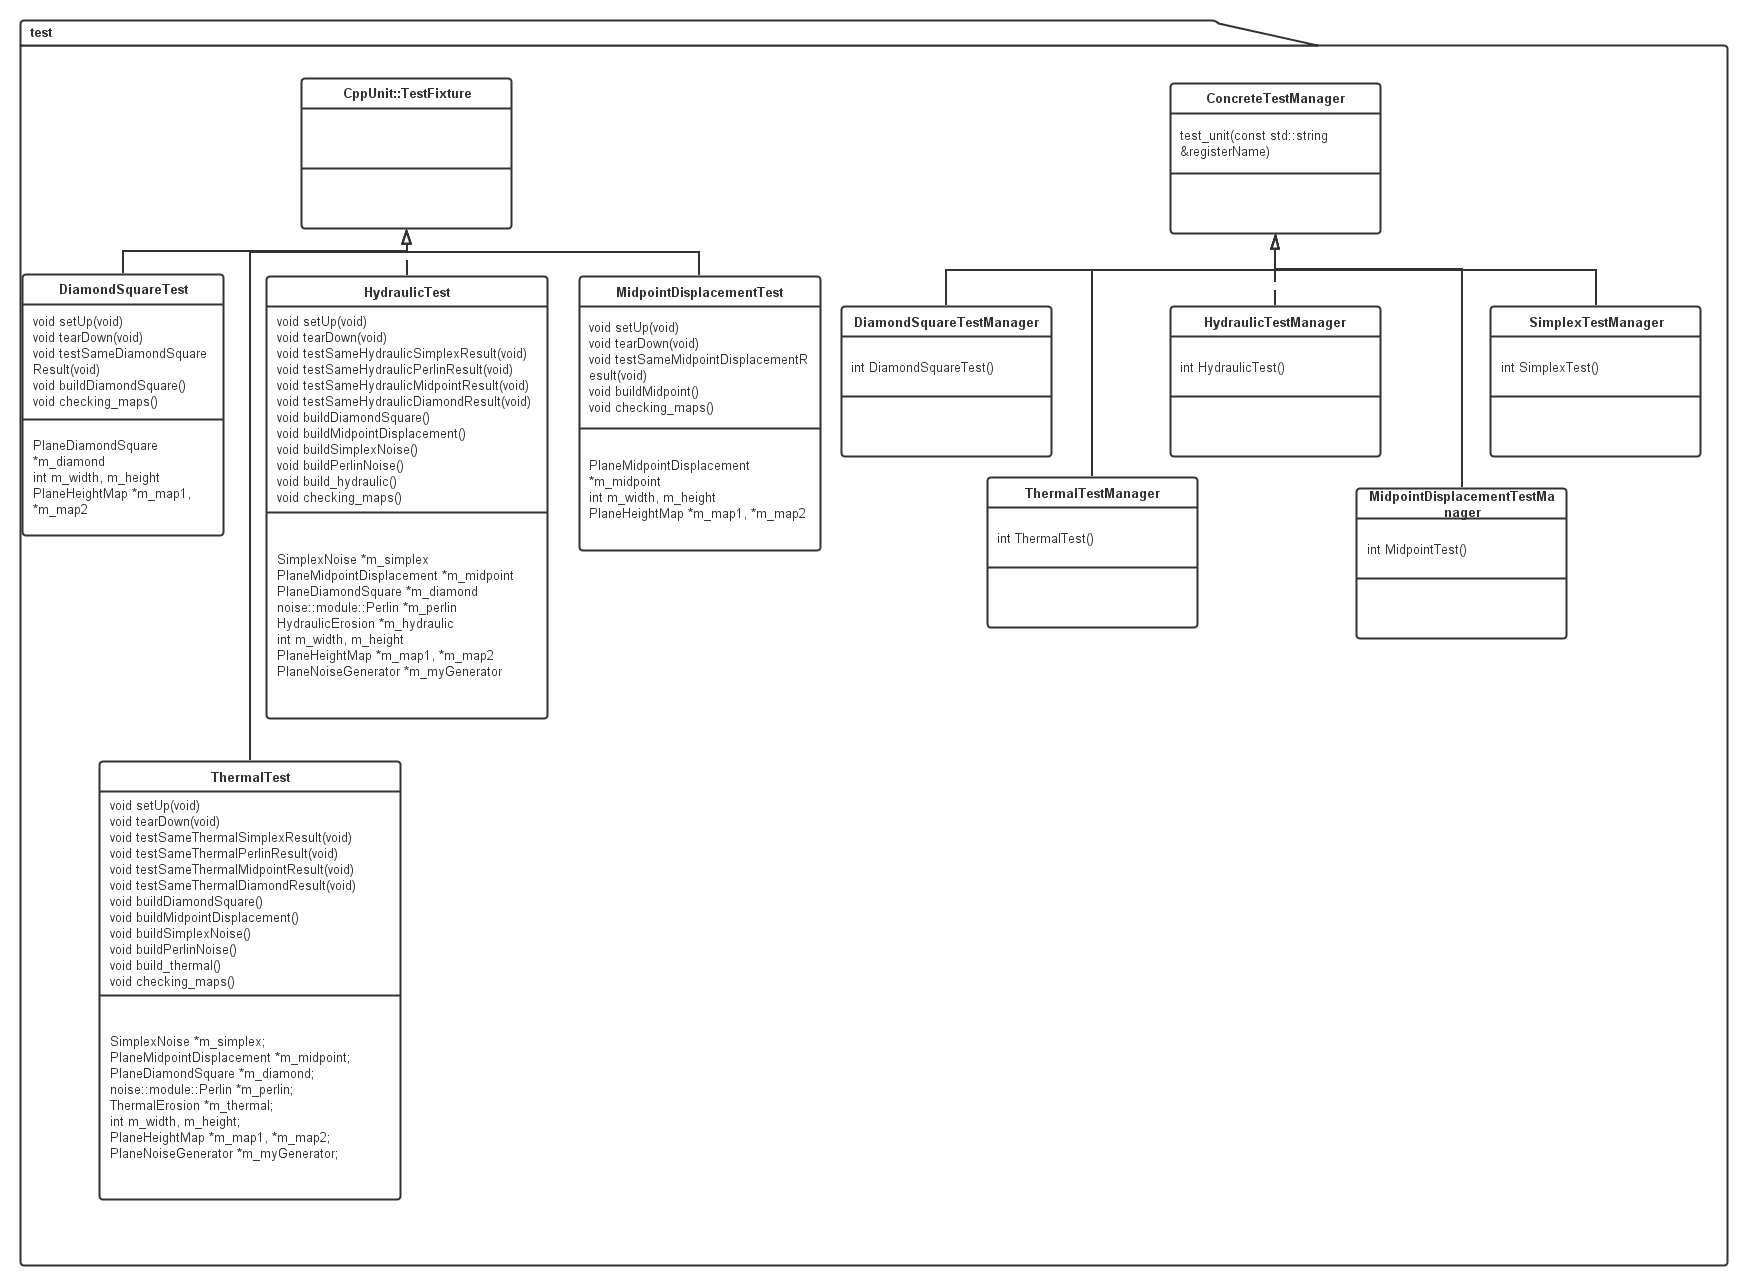
\includegraphics[width=20cm]{resources/Test_package_v2.png}
        \caption{Digramme de classe des Tests}
        \label{fig:class-diagram-test}
\end{sidewaysfigure}

Chaque méthode testée possède ses propres classes :
\begin{itemize}
 \item un manager. Il sert à remplir le registre de cppunit dédié à la méthode de génération en cours de test.
 Dans ce registre dédié, il est possible de rajouter plusieurs classes de tests pour une même méthode de génération 
  (exemple : DiamondPerf, DiamondPersistance, etc);
 \item les classes de test. Chaque classe enchaîne les tests \textit{via} les macros de cppunit.
\end{itemize}

\subsection{Classes utilitaires}
Ces classes sont des structures de données implémentées dans l'objectif de simplifier le code des 
sources.




\chapter{Résultats}

\section{Générations de Bruits}

\subsection{Bruit de Perlin (figure~\ref{fig:perlin_ref})}
Le bruit de perlin est obtenu \textit{via} l'utilisation de LibNoise.

\begin{figure}[!ht]
    \begin{center}
	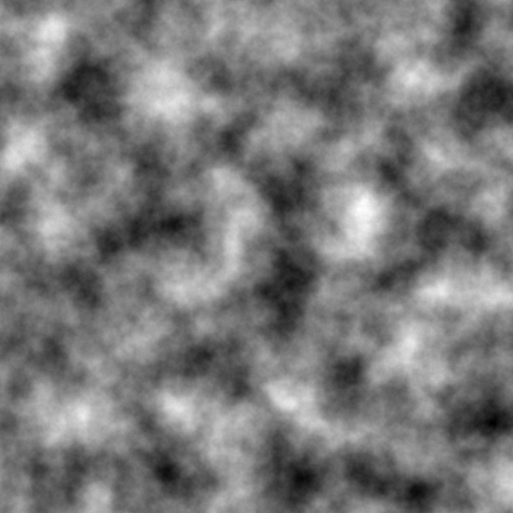
\includegraphics[width=5cm]{resources/perlin_ref.png}
        \caption{Bruit de Perlin}
        \label{fig:perlin_ref}	
    \end{center}
\end{figure}


\subsection{Bruit de Simplex (figure~\ref{fig:simplexnoise})}
Le bruit de simplex a été implémenté et permet d'obtenir des résultats satisfaisant. 
On remarque un effet de répétition et une faible variation locale de nuances (Contrairement au bruit de Perlin de LibNoise).
Cela est dû à un choix d'implémentation. Effectivement, nous sommes restés à une implémentation assez basique du bruit de Simplex.
Cela signifie que, contrairement à LibNoise, nous n'avons pas itéré N fois le bruit avec différentes amplitudes et fréquences.
Effectivement, le calcul des octaves est un ajout provenant de Fractional Brownian Motion.

\begin{figure}[!ht]
    \begin{center}
	
\includegraphics[width=10cm]{resources/simplexnoise.png}
        \caption{Bruit de Simplex}
        \label{fig:simplexnoise}
    \end{center}
\end{figure}

\section{Générations par méthodes Fractales}

\subsection{Midpoint Displacement (figure~\ref{fig:midpoint-displacementRef})}
Cette méthode fractale a été la première à être implémentée. Elle augmente la hauteur des points de 
façon progressive en partant du centre de la carte. Ainsi, on peut voir qu'il n'existera jamais de 
variation brutale des hauteurs avec cet algorithme. Ceci s'explique par sa méthode de calcul de la hauteur 
pondéré par les points adjacents.

\begin{figure}[!ht]
    \begin{center}
	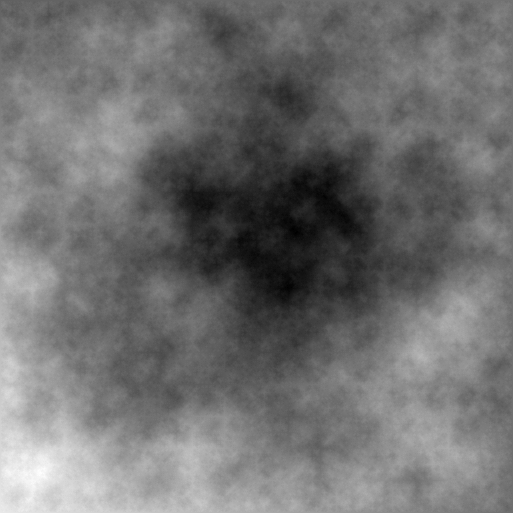
\includegraphics[width=5cm]{resources/midpoint_ref.png}
        \caption{Midpoint Displacement}
        \label{fig:midpoint-displacementRef}
    \end{center}
\end{figure}

\subsection{Diamond-Square (figure~\ref{fig:diamond_ref})}
Contrairement à Midpoint displacement, Diamond-Square propose plus de motifs mais cette méthode se 
base sur un calcul de moyennes avec une pondération par rapport aux hauteurs précédentes. 

\begin{figure}[!ht]
    \begin{center}
	
\includegraphics[width=5cm]{resources/diamond_ref.png}
         \caption{Diamond-Square}
         \label{fig:diamond_ref}
    \end{center}
\end{figure}

\section{Modèles d'érosions}
Deux modèles d'érosions sont présents dans la bibliothèque. 
L'une se nomme thermal erosion tandis que l'autre se nomme hydraulic erosion.
Les deux doivent méthodes modifient directement une carte d'élévation généré avec les méthodes cités précédemment.

\subsection{Erosion thermique (figure~\ref{fig:perlin_ref_thermal})}
L'érosion thermique simule la dégradation des reliefs avec la chute de matériaux 
vers le niveau le plus bas. Ainsi, une sensation de floue apparaît aux bordures des hauteurs.
Cet algorithme se base sur des comparaisons locales de la carte d'élévation pour altérer la hauteur de chaque sommet.
On peut voir les résultats obtenus sur le bruit de perlin ainsi que sur celui de simplex assez clairement.
On note également que la cohérence des cartes d'élévations sont les mêmes avec ou sans érosion thermique.
Cela signifie que la modification des hauteurs se calque bien sur un modèle de génération
d'où l'idée de ne pas faire un générateur d'érosion par type de carte d'élévation.

\begin{figure}[!ht]
  \begin{center}
	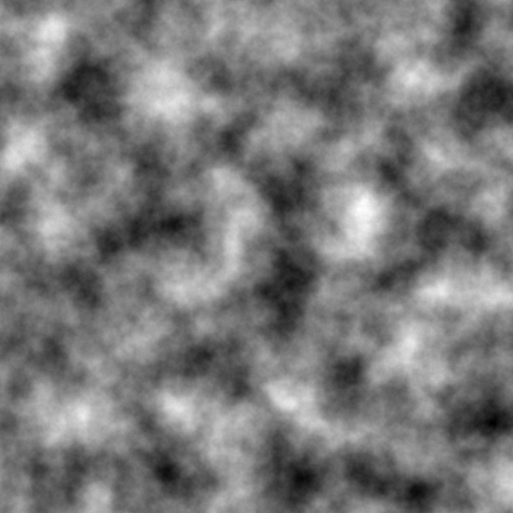
\includegraphics[width=5cm]{resources/perlin_ref.png}\hfill
	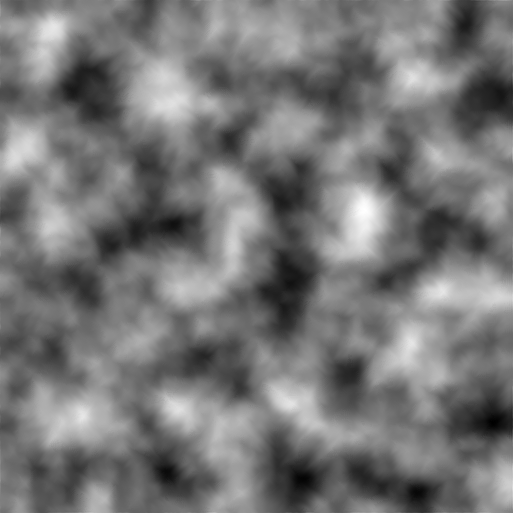
\includegraphics[width=5cm]{resources/perlin_thermalerosion.png}\hfill
        \caption{Bruit de Perlin sans érosion (gauche) et avec érosion thermique(droite)}
        \label{fig:perlin_ref_thermal}
        %%\label{fig:perlin_thermal}
        %% \caption{Bruit de Perlin avec érosion thermique}
   \end{center}
\end{figure}


\subsection{Erosion hydraulique (figure~\ref{fig:perlin_ref_hydraulic})}
L'érosion hydraulique simule plusieurs phénomènes à faible conséquence.
Effectivement, le but de ce modèle est d'apporter des 
modifications uniformes sur la carte donc la nécessité de ne pas trop accentuer des zones plus que d'autres.
Tout comme l'érosion thermique, on peut voir que l'algorithme se calque sur la carte d'élévation.

\begin{figure}[!ht]
  \begin{center}
	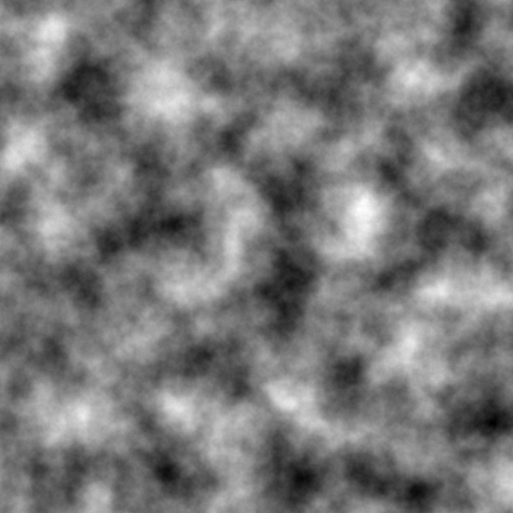
\includegraphics[width=5cm]{resources/perlin_ref.png}\hfill
	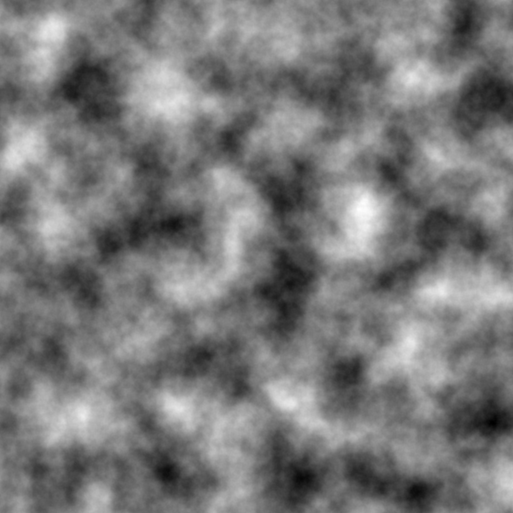
\includegraphics[width=5cm]{resources/perlin_hydraulicerosion.png}\hfill	
        \caption{Bruit de Perlin sans érosion (gauche) et avec érosion hydraulique(droite)}
        \label{fig:perlin_ref_hydraulic}
        %%\label{fig:perlin_thermal}
        %% \caption{Bruit de Perlin avec érosion thermique}
   \end{center}
\end{figure}

\section{Raffinement}
Il a été possible de raffiner localement une carte d'élévation en sélectionnant une zone de la carte.
Il ne s'agit, pour l'instant, que de modifier la valeur de pixels déjà présents. 
Nous n'avons pas encore implémenté de structures de données 
tels que les Quad-Tree pour augmenter le nombre de pixels sur une partie de la carte 
et donc augmenter le niveau de détail d'une zone donnée.

\section{Exports}
L'export des cartes d'élévations s'effectue sous différents formats : .pgm, .bmp et .ter.
L'export au format .pgm est relativement simple à mettre en place. 
Néanmoins, l'implémentation de celui-ci n'était pas spécifié dans le cahier des charges. 
Nous avons décidé d'implémenter cet export pour tester rapidement nous cartes d'élévation. 
Le format .bmp est très utilisé par les divers logiciels existants pour 
l'import et l'export d'une carte d'élévation. Le format .ter nous a permis de lire les cartes
d'élévation sous Terragen 3.
Les trois méthodes utilisent tous la même base de code c'est-à-dire qu'il y a une détection des valeurs 
maximale et minimale de la carte d'élévation dans l'objectif d'établir une échelle de gris.

\subsection{Format .pgm}
Nous n'avons pas eu besoin de bibliothèques particulière lors de l'implémentation de cet export.
Les résultats des tests concernant la cohérence des cartes d'élévation ainsi que les résultats
précédemment évoqués utilisent ce format d'export.

\subsection{Format .bmp}
Les images exportés au format .bmp sont les mêmes que celles au format.pgm. 
Ainsi, nous sommes sûr que l'export sur ce format est opérationnel.

\subsection{Format .ter}
L'export du fichier au format .ter nécessite d'écrire des en-têtes pour décrire les caractéristiques 
de la carte d'élévation. Enfin, les hauteurs de la carte d'élévation sont écrites en fin du fichier .ter.

\section{Compilation}
\subsection{Organisation}
Les fichiers du projet ont été séparés dans différents répertoires :
\begin{itemize}
 \item src/. Ce répertoire contient les fichiers sources du projet;
 \item test/. Ce répertoire contient les fichiers tests;
 \item samples/. Ce répertoire contient les exécutables produits lors de la compilation;
 \item doc/. Ce répertoire contient la documentation générable par doxygen.
\end{itemize}
Chaque répertoire possède un Makefile et un Makefile, situé à la racine du projet, permet de lire ces derniers.

\subsection{Utilisation}
La première etape est de faire \emph{./autogen.sh} et \emph{./configure} dans l'objectif de configurer et créer les fichiers
 makefile prêt. Ensuite, il est possible d'effectué différents type de \emph{make} :
 \begin{itemize}
  \item \emph{make} puis le nom de l'exécutable dans le dossier samples;
  \item \emph{make check} pour effectuer des tests;
  \item \emph{make doc} pour générer la documentation.
 \end{itemize}


%%\subsection{Format .obj}

\chapter{Qualité}
La qualité d'un programme est une grande valeur ajoutée à tout projet. Les critères qualités considérés pour ce projet sont les suivants :
\begin{itemize}
  \item les tests. Effectivement, les tests permettent de certifier certains comportement du programme.
  Nous avons choisi des tests à granularité faible (tests unitaires) avec des assertions.
  \item analyse du code.
  \item gestionnaire de projet.
  \item une documentation.
\end{itemize}


\section{Tests}

Les tests ont été effectués à l'aide de deux outils. \\
Le premier est la bibliothèque de tests cppunit. 
Celle-ci offre diverses méthodes pour lancer des pipelines de tests. 
Nous avons réaliser des tests dits de Boite Noire avec cette bibliothèque. 
Le but est que ces tests ne soient pas intrusifs dans le code.
Pour utiliser les tests, il suffit de saisir la commande \emph{make check} à la racine du code.

\subsection{Tests de persistances}
Le minimum est d'effectuer des tests de persistances pour chaque algorithme. 
En effet, nous utilisons des graines de générations ainsi que des génénateurs pseudo-aléatoires. \\
La stratégie de comparaison est la suivante :
\begin{itemize}
 \item préparation du test \textit{via} la méthode setUp(). 
 Il s'agit de construire tous les objets communs aux différents tests. 
 Il est évident que les objets initialisés sont corrects car la logique admet que Faux implique n'importe quoi.
 \item appel des différentes méthodes de tests \textit{via} les macros de cppunit. 
 Chaque macro appelle une fonction test qui exécute elle-même un test logique (Assertion).
 Ce dernier compare les hauteurs de deux objets heightmap point par point. 
 \item terminaison du test avec la méthode tearDown().
\end{itemize}

\subsection{Tests de l'existant}
La cohérence de nos résultats ont été vérifiés en les comparant avec un équivalent de l'existant.
Pour le bruit de Perlin, nous postulons que les résultats sont cohérents. Effectivement,
ces deux méthodes de génération sont issues de LibNoise.
Pour les autres bruits et méthodes fractales, il existe un grand nombre de variantes donc il est difficile
de comparer le résultat obtenu avec celui existant. Néanmoins, il a été possible d'établir des 
critères de Résultats Attendus en se basant sur les caractéristiques principales des bruits :
\begin{itemize}
 \item bruit de simplex: il phénomène de répétition à grande échelle 
 avec des regroupements de pixels de hauteurs équivalentes;
 \item érosion thermique et hydraulique : apparition d'un flou en bordure des hauteurs avec des variations de hauteurs à ces niveaux;
 \item midpoint displacement et diamond square : les heightmap sont très structurés avec des dégradés très doux 
 ce qui est aussi visible sur d'autres versions de midpoint displacement et diamond square.
\end{itemize}

\section{Analyse du code}

\subsection{Statique}
CppCheck est sous Licence GPL et est suffisant pour l'analyse statique du code que nous désirons faire.
Cet outil permet de repérer les erreurs de conception de chacune des classes non détectable par 
le compilateur g++. Ainsi, il aide à développer une architecture plus propre et plus cohérente.

\subsection{Dynamique}
Valgrind est un profileur de code. Il nous a servi à détecter les fuites mémoires présents dans le code.

\section{Gestionnaire de projet}
Un projet fonctionnel passe par une gestion rigoureuse du code et un système de communication efficace.
\subsection{Gestionnaire de version}
Gît et Subversion ont été tous les utilisés lors de ce projet. Gît pour toutes les révisions et 
Svn, pour des versions stables, lors du partage avec les encadrant du projet.
\subsection{Communication}
Trello est couramment utilisé dans le cadre de projet en groupe restreint. Il se base sur un système
de Post-It avec des assignations et des dates.
Il nous a servi à planifier les tâches (code, rapport et réunions).


\section{Documentation}
La documentation permet une meilleur compréhension du code et de l'architecture logicielle.
Nous avons utilisé le gestionnaire de documentation Doxygen car celui-ci est sous Licence GPL
et est performant. Toutes les classes, méthodes et attributs du projet (ainsi que les tests) ont été commentés.
Pour générer la documentation, il faut réaliser un \emph{make doc}.



\chapter{Perspectives}
Les délais ne nous ont pas permis de mener à terme les objectifs que nous nous étions fixé. 
Aussi il sera possible d'apporter d'autres amélioration au programme.

\section{Atteindre les objectifs fixés}

\subsection{Prioritaires}

\subsubsection{Algorithmes}
Certains algorithmes n'ont pas été implémentés comme Fractional Brownian Motion. Même si ce dernier est 
simple, nous nous sommes concentrés sur les autres algorithmes tels que les érosions. 
Pour produire Fractional Brownian Motion, il sera possible d'utiliser certains modules de LibNoise
(module d'ajout, etc). Et cela sera possible car nos bruits héritent de LibNoise (\textit{via} NoiseBase).
\subsubsection{Maillage et sphère}
Les maillages triangulaires et hexagonaux ne sont pas présents mais il serait intéressant de les
implémentés. Les sphères pourraient être conçues en partant d'un carte cubique ou d'un isocahèdre.
\subsubsection{Raffinement locale}
Un raffinement existe mais il ne permet pas de zoomer sur une zone de la carte. Il faudrait 
utiliser les Quad-Tree pour cela. Chaque noeud du Quad-Tree contiendrait un face avec les vertex de la grille.
Chaque fils de la grille serait une partie de la grille subdivisée (tesselation des grilles). Ainsi, il serait possible d'obtenir :
\begin{itemize}
 \item quatre fils pour les grilles carrées et triangulaires;
 \item sept fils pour les grilles hexagonales.
\end{itemize}

\subsection{Secondaires}

\subsubsection{Implémentation d'un visualisateur}
Il serait intéressant d'implémenter le visualisateur proposé sur le cahier des charges. De plus, 
l'intégration avec le Quad-Tree permettrait d'obtenir une génération procédurale temps-réel avec des fonctions de zoom.

\section{Amélioration des tests}
Les tests unitaires effectués, jusqu'à présent, ne couvrent que les méthodes de générations. Aussi, 
les grilles carrées, pour les cartes d'élévation planaires, n'ont pas été testées de façon approfondi. 
Aussi, les exportations pour Blender3D sont à tester correctement. Effectivement, nous nous sommes uniquement assurés 
de la lisibilité des fichiers exportés sur Blender3D.

\section{Diminution du temps de calcul}
Avec l'intégration d'un visualisateur, il va nécessairement falloir gagner du temps sur le calcul pour avoir un rendu temps-réel.
Ainsi, l'utilisation du GPU est préférable au CPU. Il faudrait utiliser CUDA et/ou les shaders d'OPENGL pour effectuer
les calculs sur le GPU.

\section{Interopérabilité}
L'un des concept de ce projet est l'importation et l'exportation des cartes d'élévation. En allant plus loin,
il serait possible de :
\begin{itemize}
 \item adapter les cartes d'élévation pour d'autres logiciels;
 \item proposer des classes de conversions de cartes d'élévation entre logiciels;
 %%TODO\item .  
\end{itemize}


\bibliographystyle{alpha}
\bibliography{report-1}

\end{document}

